%! TeX program = pdflatex
\documentclass{article}
\usepackage[english]{babel}
\usepackage[utf8]{inputenc}
\usepackage{amsmath}
\usepackage{amssymb}
\usepackage{minted}
\usepackage{listings}
\usepackage{xcolor}
\usepackage{algorithm}
\usepackage{algorithmicx}
\usepackage{hyperref}
\usepackage{graphicx}
% \usepackage{natbib}
\usepackage{subcaption} 
\usepackage{graphicx}
% \usepackage{url}
\usepackage{algorithm}% http://ctan.org/pkg/algorithms
\usepackage{algpseudocode}% http://ctan.org/pkg/algorithmicx
% \usepackage{tikz-cd}
\usepackage{listings}
\usepackage{xcolor}
% \usepackage[colorlinks, linkcolor = blue, citecolor = magenta]{hyperref}
\usepackage{float}
\usepackage{placeins}
\usepackage{pgfplots}
\usepackage{tikz}
\usepackage[margin=1in]{geometry}
\pgfplotsset{compat=1.18}
\usepackage{tikz}
\usetikzlibrary{positioning}
% % \usepackage{minted}
\usepackage{float}
% \usetikzlibrary{shapes, arrows, positioning}
% \lstset{ 
%     language=Python,                 % the language of the code
%     basicstyle=\ttfamily\small,      % the size of the fonts that are used for the code
%     numbers=left,                    % where to put the line-numbers
%     numberstyle=\tiny\color{gray},   % the style that is used for the line-numbers
%     stepnumber=1,                    % the step between two line-numbers. If it's 1, each line will be numbered
%     numbersep=5pt,                   % how far the line-numbers are from the code
%     backgroundcolor=\color{white},   % choose the background color. You must add \usepackage{color}
%     showspaces=false,                % show spaces adding particular underscores
%     showstringspaces=false,          % underline spaces within strings
%     showtabs=false,                  % show tabs within strings adding particular underscores
%     frame=single,                    % adds a frame around the code
%     rulecolor=\color{black},         % if not rolframe-color may be changed on line-breaks within not black text (e.g. comments (green here))
%     tabsize=4,                       % sets default tabsize to 4 spaces
%     captionpos=b,                    % sets the caption-position to bottom
%     breaklines=true,                 % sets automatic line breaking
%     breakatwhitespace=false,         % sets if automatic breaks should only happen at whitespace
%     title=\lstname,                  % show the filename of files included with \lstinputlisting; also try caption instead of title
%     keywordstyle=\color{blue},       % keyword style
%     commentstyle=\color{green},      % comment style
%     stringstyle=\color{red},         % string literal style
%     escapeinside={\%*}{*)},          % if you want to add LaTeX within your code
%     morekeywords={*,...} 
% }            % if you want to add more keywords to the rol\newenvironment{notation}
\newtheorem{remark}{Remark}
\newtheorem{definition}{Definition}
\newtheorem{property}{Property}
\newcommand{\DoParallel}[1]{\textbf{parallel do} \{#1\}}
\newcommand{\pder}[2]{\frac{\partial #1}{\partial #2}}

\title{COLMENA Prototype for ANDES}
\author{Pablo de Juan Vela $^{1}$ \\
        \small $^{1}$eRoots, Barcelona, Spain \\
}
\date{\today}

\usepackage[style=ieee]{biblatex}
\addbibresource{ref.bib}
\setlength{\parskip}{1em} 
\begin{document}
\maketitle

\section{Introduction}

This first prototype tries to showcases the main capabilities of COLMENA applied to power systems. The prototype aims to use the different tools of COLMENA to react to changes in the grid and apply the necessary changes through the intermediary of the roles previously described. The focus is therefore in the roles themselves but also how the roles react to changes in the grid and how these reactions result in better KPIs for the whole grid. In this prototype presentation we will give an overview of the grid used, the roles and the agents present in the simulation and finally the specific ways that the roles activate through KPI to change the grid. The proptotype's code and implementation can be seen in the git repository \cite{git:eroots}.     

\section{Grid Definition}

We chose a modified version of the IEEE39 \cite{grids:ieee39} that will serve as a testing ground for the prototype. The original grid consists of 39 buses, 10 synchronous generators and 19 loads. In order to better demonstrate the capabilities of COLMENA we switch the generators to converters that can  be operated in GFM(mode) or GFL(mode). The converter in GFM mode simulates a spinning mass mirroring the behavior of a generator. We define the grid as a dynamic system that evolves over time.
\begin{figure}[h]
    \centering
    \begin{center}
        \includegraphics[width=0.8\textwidth]{plots/IEEE39 (1).png}
    \end{center}
    \caption{Your caption here}
    \label{fig:your_label}
\end{figure}

\subsection{Grid Dynamics}

\subsubsection*{Changes in the Grid's topology}

This type of changes are the ones directly affecting the connection status of an electric device. For example, switching a generator off or having a line failure.

\subsubsection*{Change in Modes}
A change in mode changes the internal definitions and states of the device. Although the power exchanges in the bus stay similar just after the change the control logic behind it can be completely changed.

\subsubsection*{Change in devices Set Points}

Here the control logic is not directly changed but some reference values that describe the desired steady state values. For example a reference voltage value for a converter.

\section{Roles \& Agents}


\subsection{Agents}
In the simulation we consider 6 different agents. Specifically, three of the agents are coupled to converter devices, two of them are coupled to generators and one of them is coupled to a load. At initialization, the agent receive their coupled device data from Andes. The pairings are defined before the simulation starts. We define the agents with the following hardware tags:

\begin{itemize}
    \item \textbf{Generator Compatible}
    \item \textbf{Converter Compatible}
    \item \textbf{Load Compatible}
\end{itemize}

We use these different hardwares so that an agent monitoring a specific type of device can only execute the roles compatible with that device. For example, the LoadSheddingRole only makes sense if executed in an agent that is monitoring a Load device. Therefore, adding both the hardware to the agent definition and the requirement to the role definition ensures that the roles activated in that agent are compatible with the device.

Also, the agents present in the prototype are always activated with a LAZY policy. When running an agent with a LAZY policy, the agent only executes roles with KPIs that are being broken. This ensures that the roles are only activated when they are actually needed to correct a broken KPI. 

\subsection{Roles}

For this simulation use case we include different roles that participate in the frequency response. The different roles govern the agent's behaviors during the simulation. It is also through these roles that the agents can modify the grid.  

\begin{table}[h]
    \centering
    \small % Reduce font size
    \renewcommand{\arraystretch}{1.2} % Adjust row spacing
    \begin{tabular}{|p{3cm}|p{3cm}|p{4cm}|p{4cm}|} % Adjusted column widths
    \hline
    Role & Requirement & Behavior & KPI \\
    \hline
    Monitoring & None & Monitors its device's data & NA\\
    Load Shedding & Load Compatible & Reduces the device's load & $\omega \notin [\omega_{min},  \omega_max]$\\
    Automatic Secondary Response & Generator or Converter Compatible& Activates automatic response & $\omega \notin [\omega_{min},  \omega_max]$\\
    GFM & Converter Compatible & Activates the GFM Role & $\omega \notin [\omega_{min},  \omega_max]$\\
    \hline
    \end{tabular}
    \caption{Summary of Roles}
    \label{tab:roles}
\end{table}

\subsubsection*{Monitoring Role}

This role runs persistently in every agent that is paired with a physical device. When this role initializes it stores the initial values of the devices states. Then it sends periodic requests to the ANDES simulation to keep the stored values updated. Additionally, it publishes the key metrics that are important for the service in COLMENA. In this case the published metrics are the voltage of the bus the device is connected to and the generator's frequency if the agent monitors a generator. We aim to run this run continuously, this would mean syncing the stored data with a high frequency. In order to execute the role continuously we define the role with a mock KPI that is always broken, this ensures the role is always activated. In the future we envision changing this when the functionality is available.   

\subsubsection*{Automatic Generation Control}

This role is activated when the frequency is seen by the agent is out of the admissible interval. This role is only compatible with devices injecting power to the grid such as generators and converters. The rol defines a PI controller with a feedback loop that adjust the power delivered by the device. The role reads the frequency value from the agent data and then sends the change in power to the device as a change of parameter.

\subsubsection*{GFM Role}

This role changes the operation mode of GFL converters to GFM to converters. It is activated when the frequency seen by the device is out of the admissible interval. When the role ends its execution the agent changes the mode of the converter back to GFM.

\subsubsection*{Load Shedding Role}

This role is engaged when the frequency is out of the admissible interval and the Automatic Generation Response has been running in a nearby generator for at least 30 seconds. When activated the agent reduces the consumed load linearly, when the role is disengaged the change is reversed.


\section{Service Prototype}

\subsection*{Service Description}

The prototype is simulating an electrical grid with multiple perturbations that happen over the simulation's time. The service objective is to maintain the frequency of the grid generator's inside an acceptable range. The acceptable range is defined as $\omega_{acceptable}[\omega_{min}, \omega_{max}] = [0.9999, 1.0001]$. The KPI associated to the frequency metric ($\omega$) is the KPI used for activating the GridFormingRole and AutomaticGenerationControl role. The objective of this prototype is to show that the activation if these roles correct the deviation on the metric ($\omega$).  

The prototype deploys 4 agents in separate dockers containers. Two of them are paired to transformers and the other two to generators. The roles associated with the transformers are able to change the control of the transformer from GFL to GFM while the Automatic Generation Control is able to adapt the power being outputed by the generator online using a Proportional Integral controller.
 
\subsection{Andes Interaction}

The grid is simulated through the ANDES package. The Grid is initialized with the values from the power flow results. Afterwards Andes is deployed in a port using Flask. The different agents can request information from ANDES using the appropriate HTTP requests. Changing the grid's parameter follows a similar procedure. At any point during the simulation the agents can send the data for a change in the grid. This change is received by the Flask app and reflected just afterwards in the simulation. And since the ANDES simulation and COLMENA have the same clock by running in parallel the change requested by COLMENA is reflected at the appropriate time in ANDES.  

\begin{algorithm}
    \caption{Grid Simulation}
    \label{algo:COLMENAANDES}
    \begin{algorithmic}[1]
        \State Initialize grid states $x$ to $x_0$ with the Power Flow results.
        \For{agent in Agents}
            \For{device in controllable devices}
                \If{device is not controlled}
                    \State Pair agent to device
                \EndIf
            \EndFor
        \EndFor
        \While{not Stop}
            \DoParallel
                \State Receive Parameter Changes
                \State Run Simulation Online (steps of $\Delta$ t = 0.1s)
        \EndWhile
        \State Finalize the result.
    \end{algorithmic}
\end{algorithm}

\begin{figure}[h]
    \centering
    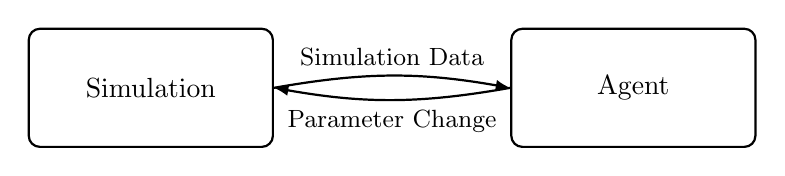
\begin{tikzpicture}[node distance=6cm and 3cm, >=latex, thick]

        % Define smaller nodes with rounded corners
        \node[draw, rectangle, rounded corners, minimum width=3.1cm, minimum height=1.5cm, align=center] (sim) {Simulation};
        \node[draw, rectangle, rounded corners, minimum width=3.1cm, minimum height=1.5cm, align=center, right=of sim] (agent) {Agent};

        % Adjusted rounded arrows with different start and end positions
        \draw[->, rounded corners] (sim.east) to[out=10, in=170] node[above, font=\small] {Simulation Data} (agent.west);
        \draw[<-, rounded corners] (sim.east) to[out=-10, in=-170] node[below, font=\small] {Parameter Change} (agent.west);
    \end{tikzpicture}
    \caption{Interaction between the simulation and agent.}
    \label{fig:sim_agent_interaction}
\end{figure}

In this use case the agents only receive data from the device their paired to and they only change the parameters of the same device. This is a constraint that comes from the agent-device pairing that we envisioned in the beginning. 

\subsection{Simulation Setup}

The grid simulation starts from a steady-state solution that was computed beforehand. In order to model the dynamic changes in the grid we introduce multiple changes manually. These changes are variable loads simulating the variability of the consumption in electric power and also line failures. These changes introduce perturbations to the grid that will make the agents respond. The objective is to showcase the different actions that the agent will perform to the grid to maintain the grid's frequency stability. The simulation runs for $55$s and observe the different transient responses compared to the simulation with just the automatic response.

\begin{table}[h]
    \centering
    \begin{tabular}{|l|c|r|}
    \hline
    Perturbation & Device & Change \\
    \hline
    Line Failure & Line 2 & Line disconnected at $t =3$s\\
    Load Increase & Load 1 & Load increases 50\% at $t =18$s \\
    Load Increase & Load 2 & Load increases 50\% at $t =33$s \\
    \hline
    \end{tabular}
    \caption{Table of non-agent induced changes in the grid}
    \label{tab:example}
\end{table}
\subsection{Results}

To compare the results we use a control simulation in the same power grid and performing the same perturbation to the grid but without activating any roles. We compare the evolution of the metrics being monitored.
\begin{figure}[h!]
    \centering
    \begin{subfigure}[t]{0.48\textwidth}
        \centering
        \includegraphics[width=\linewidth]{plots/control_omega.png}
        \caption{$\omega$ evolution for control simulation.}
        \label{fig:image1}
    \end{subfigure}
    \hfill
    \begin{subfigure}[t]{0.48\textwidth}
        \centering
        \includegraphics[width=\linewidth]{plots/colmena_omega.png}
        \caption{$\omega$ evolution for COLMENA simulation.}
        \label{fig:image2}
    \end{subfigure}
    \caption{Comparison of $\omega$ evolution in control and COLMENA simulations.}
    \label{fig:two_images}
\end{figure}

As we can see in the multiple plots the metric tends to converge towards the nominal value of 1 thanks to the action of the roles. Additionally the roles activate when there exists a deviation in the metric provoked by the grid perturbations. 
\begin{figure}[h!]
    \centering
    
    % Plot 1
    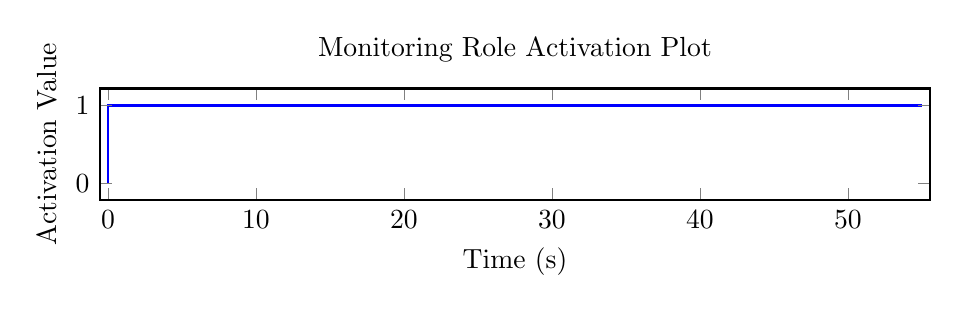
\begin{tikzpicture}
    \begin{axis}[
        width=\linewidth,
        height=3cm,
        xlabel={Time (s)},
        ylabel={Activation Value},
        ymin=-0.2, ymax=1.2,
        xmin=0, xmax=55,
        xtick={0,10,20,30,40,50},
        ytick={0,1},
        title={Monitoring Role Activation Plot},
        enlargelimits=0.01,
        axis on top,
        thick
    ]
    \addplot [
        const plot,
        draw=blue,
        line width=1pt
    ] coordinates {
        (0,0) (0,1) (55,1)
    };
    \end{axis}
    \end{tikzpicture}
    
    \vspace{0.5cm}
    
    % Plot 2
    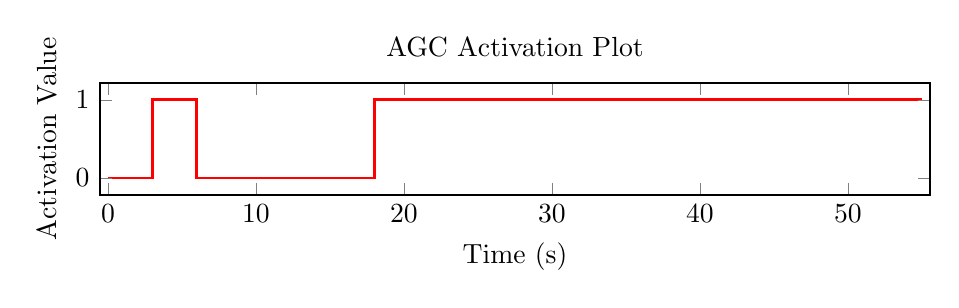
\begin{tikzpicture}
    \begin{axis}[
        width=\linewidth,
        height=3cm,
        xlabel={Time (s)},
        ylabel={Activation Value},
        ymin=-0.2, ymax=1.2,
        xmin=0, xmax=55,
        xtick={0,10,20,30,40,50},
        ytick={0,1},
        title={AGC Activation Plot},
        enlargelimits=0.01,
        axis on top,
        thick
    ]
    \addplot [
        const plot,
        draw=red,
        line width=1pt
    ] coordinates {
        (0,0) (3,0) (3,1) (6,1) (6,0) (18,0) (18,1) (55,1)
    };
    \end{axis}
    \end{tikzpicture}
    
    \vspace{0.5cm}
    
    % Plot 3
    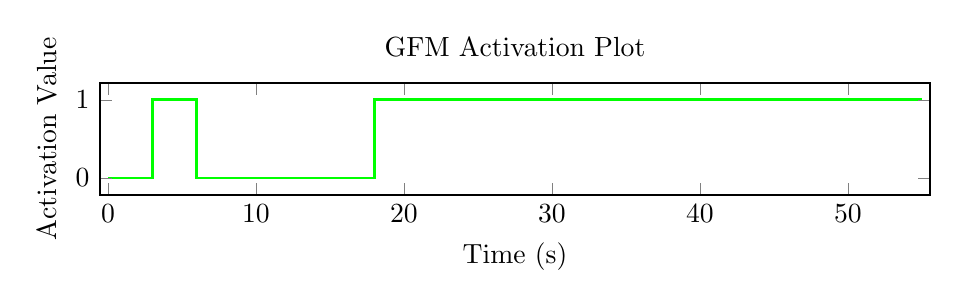
\begin{tikzpicture}
    \begin{axis}[
        width=\linewidth,
        height=3cm,
        xlabel={Time (s)},
        ylabel={Activation Value},
        ymin=-0.2, ymax=1.2,
        xmin=0, xmax=55,
        xtick={0,10,20,30,40,50},
        ytick={0,1},
        title={GFM Activation Plot},
        enlargelimits=0.01,
        axis on top,
        thick
    ]
    \addplot [
        const plot,
        draw=green,
        line width=1pt
    ] coordinates {
        (0,0) (3,0) (3,1) (6,1) (6,0) (18,0) (18,1) (55,1)
    };
    \end{axis}
    \end{tikzpicture}
    
    \caption{Three binary signals switching from 0 to 1 at 4.5s, without fill}
\end{figure}
    

\section{Milestone Review}

\subsection*{Milestone 1}

The prototype  integrates the implementation of the first algorithms developed within the project. We validate the applicability of the technology in a pilot setup. The analysis includes dynamical simulations of power system, which requires more than just referencing the magnitudes controlled by power converters: it also involves the control loops themselves, such as the ones controlling the power output of generators through roles. These directly influence the system's dynamic behavior.

To this end, the prototype incorporates initial heuristics and methodologies that enable transitions between different converter operation modes, such as from grid-following to grid-forming. The completion of this milestone confirms that a first version of the prototype is operational and already capable of executing this type of flexible control logic within the environment.

\subsection*{Milestone 2}

Following the internal validation of the initial prototype, this milestone corresponds to the publication of the first version of the pilot in an open-access repository such as GitHub or GitLab. The purpose is to facilitate transparency, community engagement, and external testing.

The codebase relies on open-source Python packages for static and dynamic power system analysis. The main package used is ANDES \cite{article:andes} that uses a free software copyleft license GPLv3 which permits modifications of any original work and ensures the full work is still published in the same license, the changes can however be copyrighted. The repository has been prepared and published \cite{git:eroots}, fulfilling the objectives of this milestone.

\subsection{Conclusion}

This prototype is a first step for creating an interesting test case for COLMENA in power grids. Indeed, we can see that the different roles are activated when the KPIs are violated and then the metrics come back to more desirable values. This behavior is seen thanks to changes in the grid that the roles perform in the grid. The COLMENA controlled prototype sees overall less violated KPIs than the control. 

The next steps in improving this prototype is using the new COLMENA functionalities to be able to be more precise with the use of metrics and KPIs. This means being able to define KPI that are more adequate to the roles we used. For example, instead of aggregating the KPIs in the whole grid we could aggregate the KPIs for specific areas and agents, so only the concerned agents would execute the roles needed. Similarly, using more complicated rules to combine the activation of roles could bring greater performance. For example, combining cost and operative KPI.

On another the new COLMENA capabilities also enable more inter role communication. This inter role communication can enable more complex operations on the grid. We envision for example roles that could control specific areas on the grid and communicate their data to develop a distributed control based on Model Predictive Control. 
\nocite{*}
\printbibliography
\end{document}